\chapter{Annexes du chapitre 4}\label{annexe-3}
\dochaptoc

\section{Performances de CLS sans ACP}\label{sec-perfs-without-acp}

\`A la section~\ref{sec-formulation-cls}, l'ACP a été considérée pré-traitement de l'algorithme proposé CLS. En effet, appliquer une ACP en pré-traitement présente un avantage double : cela permet d'imposer une structure faible-rang de l'image reconstruite tout en réduisant drastiquement le temps d'exécution. Dans cette même section, le risque de voir apparaître des artefacts lorsque l'estimation de la matrice de covariance est imprécise a été souligné.

Dans cette section, l'amélioration en termes de performances de reconstruction apportée par ce pré-traitement sera illustré. Pour cela, pour différents taux d'échantillonnage, l'image semi-réelle $\mathsf{R}_2^*$ est reconstruite avec CLS en le pré-traitant par ACP ou non.
%
Les performances de reconstruction en termes de SNR, aSAD et SSIM ainsi que le temps d'exécution sont donnés en fonction du taux d'échantillonnage aux figures~\ref{fig-CLS-full-a}, \ref{fig-CLS-full-b}, \ref{fig-CLS-full-c} et \ref{fig-CLS-full-d} respectivement. Pour toutes les métriques et tous les taux d'échantillonnage, appliquer une ACP en pré-traitement améliore les performances de reconstruction. De plus, cela permet de diviser le temps d'exécution par 200. Enfin, la figure~\ref{fig-CLS-full-images} montre les images reconstruites autours de trois seuils principaux lorsque l'ACP est appliquée et quand elle ne l'est pas (pour un taux d'échantillonnage de 20\%). Aucune différence visuelle ne peut être observée entre les deux procédures.
 
\begin{normalfigure*}[]
    \centering
    %
    \subfigure[Evolution du SNR avec le taux d'échantillonnage.\protect\label{fig-CLS-full-a}]{
        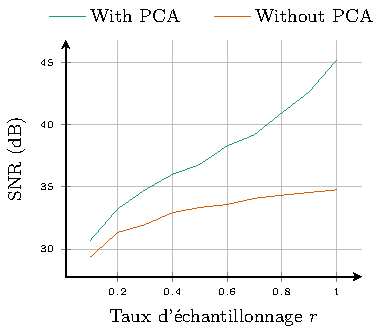
\includegraphics{img/chapitre4/figure12/perf_1.pdf}}
    \hspace{1cm}
    %
    \subfigure[Evolution du aSAD avec le taux d'échantillonnage.\protect\label{fig-CLS-full-b}]{
        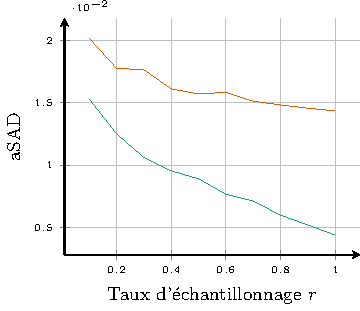
\includegraphics{img/chapitre4/figure12/perf_2.pdf}}\\
    %
    \subfigure[Evolution du SSIM avec le taux d'échantillonnage.\protect\label{fig-CLS-full-c}]{
        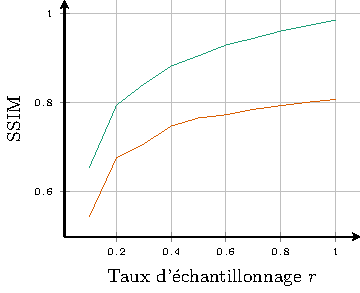
\includegraphics{img/chapitre4/figure12/perf_3.pdf}}
    \hspace{1cm}
    %
    \subfigure[Evolution du temps d'exécution avec le taux d'échantillonnage.\protect\label{fig-CLS-full-d}]{
        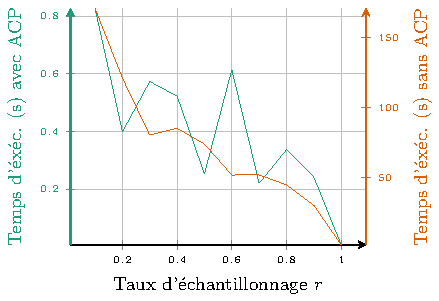
\includegraphics{img/chapitre4/figure12/perf_4.pdf}}
    %
    \caption{Performances de reconstruction et temps d'exécution en fonction du taux d'échantillonnage $r$ pour l'image semi-réelle $\mathsf{R}_2^*$ avec CLS,  avec ou sans pré-traitement par PCA.
        \protect\label{fig-CLS-full}}
\end{normalfigure*}

\begin{normalfigure*}[]
    \centering
    %
    \begin{tabular}{m{0.12\textwidth}*{3}{M{0.23\textwidth}}}
        Component&O - K&La - M\textsubscript{4, 5}&Nd - M\textsubscript{4, 5}\\
        Référence
        &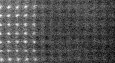
\includegraphics[width=0.22\textwidth]{img/chapitre4/figure13/img/GT_0.png}
        &
\includegraphics[width=0.22\textwidth]{img/chapitre4/figure13/img/GT_1.png}
        &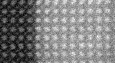
\includegraphics[width=0.22\textwidth]{img/chapitre4/figure13/img/GT_2.png}
        \\
        Avec ACP
        &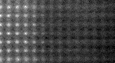
\includegraphics[width=0.22\textwidth]{img/chapitre4/figure13/img/PCA_0.png}
        &
\includegraphics[width=0.22\textwidth]{img/chapitre4/figure13/img/PCA_1.png}
        &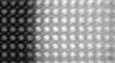
\includegraphics[width=0.22\textwidth]{img/chapitre4/figure13/img/PCA_2.png}
        \\
        Sans ACP
        &
\includegraphics[width=0.22\textwidth]{img/chapitre4/figure13/img/Full_0.png}
        &
\includegraphics[width=0.22\textwidth]{img/chapitre4/figure13/img/Full_1.png}
        &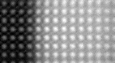
\includegraphics[width=0.22\textwidth]{img/chapitre4/figure13/img/Full_2.png}
        \\
\end{tabular}
    %
    \caption{Résultats de reconstruction de $\mathsf{R}_2^*$ avec ACP (milieu) ou sans ACP (bas) en termes de pré-traitement. Les images montrent la somme de 5 bandes autours de trois seuils caractéristiques ($\mathrm{O-K}$, $\mathrm{La-M}_{4, 5}$ et $\mathrm{Nd-M}_{4, 5}$). La référence correspond à l'image semi-réelle $\mathsf{R}_2^*$.
        \protect\label{fig-CLS-full-images}}
\end{normalfigure*}



\section{Comparaison des performances pour plusieurs taux d'échantillonnage}\label{sec-autres-taux-echantillonnage-hr}

La méthode CLS proposée peut fonctionner avec n'importe quel taux d'échantillonnage. Toutefois, si un pré-traitement par ACP est réalisé, réduire le taux d'échantillonnage peux dégrader la qualité de l'estimation de la matrice de covariance. En particulier, lorsque le nombre de pixels acquis est inférieur au nombre de bandes (\ie{}, une configuration appelée \guillemets{large $p$, small $n$}), un estimateur robuste de la matrice de covariance serait nécessaire afin de surmonter le problème d'instabilité des estimateurs conventionels~\cite{ledoit2004well}. Dans nos expériences, les images complètes sont composées de \np{10000} pixels tandis que le nombre de bandes spectrales vaut environ \np{1500}. En choisissant un taux d'échantillonnage de 20\%, nous nous assurons que le nombre de pixels acquis est au moins légèrement supérieur au nombre de bandes, ce qui garanti que l'estimation de la matrice de covariance soit un problème bien posé.

En tant que résultat complémentaire, les performances des algorithmes comparés ont été évaluées pour différents taux d'échantillonnages lors de la reconstruction de $\mathsf{R}_2^*$. Les résultats sont donnés à la \tabname~\ref{table-higher-samp-ratio}. Comme attendu, les performances de toutes les méthodes augmentent avec le taux d'échantillonnage. On peut aussi noter que l'algorithme proposé est toujours performant pour des taux d'échantillonnage faibles ou élevés (\ie{}, 5\% et 50\%).

\begin{table}[h!]
    \centering
    \subfigure[SNR - Image bruitée: 26,75\,dB.]{
        \begin{tabular}{*{6}{c}}
            \toprule
            Taux d'éch.  & 0.05 & 0.1 & 0.2 & 0.3 & 0.5\\
            \midrule
            NN&24,81&26,42&28,71&29,91&32,04\\
            3S&26,89&27,76&30,17&31,77&34,92\\
            CLS&29,31&30,84&33,15&34,56&37,10\\
            ITKrMM&29,75&31,82&33,67&34,14&34,57\\
            wKSVD&25,51&29,63&34,52&35,52&35,90\\
            \bottomrule
        \end{tabular}
    }\\
    %
    \subfigure[aSAD ($\times$100) - Image bruitée : 4,613.]{
        \begin{tabular}{*{6}{c}}
            \toprule
            Taux d'éch.  & 0,05 & 0,1 & 0,2 & 0,3 & 0,5\\
            \midrule
            NN&2,846&2,325&1,815&1,542&1,148\\
            3S&2,358&2,041&1,496&1,217&0,857\\
            CLS&1,795&1,539&1,233&1,076&0,856\\
            ITKrMM&1,662&1,406&1,253&1,198&1,163\\
            wKSVD&2,740&1,690&1,163&1,086&1,072\\
            \bottomrule
        \end{tabular}
    }\\
    %
    \subfigure[SSIM - Image bruitée : 0,460.]{
        \begin{tabular}{*{6}{c}}
            \toprule
            Taux d'éch.  & 0,05 & 0,1 & 0,2 & 0,3 & 0,5\\
            \midrule
            NN&0,233&0,425&0,635&0,720&0,823\\
            3S&0,216&0,369&0,621&0,742&0,877\\
            CLS&0,545&0,660&0,790&0,843&0,911\\
            ITKrMM&0,620&0,757&0,819&0,831&0,844\\
            wKSVD&0,499&0,717&0,841&0,858&0,866\\
            \bottomrule
        \end{tabular}
    }
    \caption{Performances de reconstruction en terme de SNR, aSAD et SSIM pour l'image semi-réelle $\mathsf{R}_2^*$ pour différents taux d'échantillonnage. Les métriques sont aussi évaluées pour l'image bruitée $\mathsf{R}_2^*$ pour servir de référence.
        \protect\label{table-higher-samp-ratio}}
\end{table}



%
\section{Estimation du paramètre de CLS à partir du niveau de bruit estimé}\label{sec-lcls-param-estim}

En s'inspirant de la stratégie décrite à la section~\ref{sec-s2n-param-tuning}, le paramètre de régularisation de CLS peut être ajusté en suivant une approche dichotomique, comme discuté à la section~\ref{sec-choix-param-CLS}. Plus précisément, l'expérimentateur a généralement une certaine connaissance de l'image à reconstruire, telle que le niveau de bruit, pouvant être estimé a priori, ou le niveau de parcimonie, \ie{}, la proportion de coefficients non-nuls dans la représentation par DCT de l'image. Cette connaissance a priori peut être utilisée afin d'évaluer la qualité de la solution $\gls{Xh}_{\lambda}$ obtenue par CLS pour une valeur donnée $\lambda$\footnote{L'indice CLS de \gls{lcls} est omis pour plus de lisibilité.} du paramètre de régularisation. En effet, le terme d'attache aux données $\frac{1}{2} \frobnorm{\gls{Yi} - (\gls{Xh}_\lambda)_{\gls{I}}}$ devrait être de l'ordre de grandeur du niveau de bruit. De plus, ce terme résiduel (resp. le terme de parcimonie $||\gls{Xh}_\lambda\Psi||_{2, 1}$)  est censé augmenter (resp. diminuer) avce le paramètre $\lambda$ de CLS. Ainsi, une recherche dichotomique peut être menée afin d'ajuster automatiquement le paramètre de régularisation. Cela consiste à exécuter l'algorithme CLS, calculer le terme d'attache aux donnée à convergence, et à ré-exécuter une nouvelle fois CLS après avoir augmenté ou diminué le paramètre de régularisation jusqu'à atteindre une valeur du terme d'attache aux données proche du niveau de bruit. Par exemple, une approche similaire a été utilisée à la section~\ref{sec-lr-param-tuning}.

Pour illustrer cela, en suivant le protocole expérimental décrit à la section~\ref{sec-experiments-hr}, CLS est utilisé afin de reconstruire l'image $\mathsf{R}_2^*$ pour une large gamme de valeurs de paramètre $\lambda$. Les performances de reconstruction en termes de SNR sont affichées à la figure~\ref{fig-lambda_estim} en fonction de $\lambda$. Sur cette figure, le paramètre ajusté à l'aide de la recherche dichotomique est indiqué par un point orange tandis que le paramètre optimal (\ie{}, celui conduisant à la meilleure reconstruction) apparaît en rouge. Ces résultats montrent que la stratégie proposée afin d'ajuster automatiquement le paramètre de régularisation donne des performances de reconstruction proches des valeurs optimales.

Notons toutefois que, pour toutes les méthodes comparées aux expériences de la section~\ref{sec-hr-results}, les performances obtenues correspondent à un choix optimal des paramètres de l'algorithme, \ie{}, permettant d'atteindre les performances optimales pour la méthode.

\begin{figure}[ht!]
    \centering
    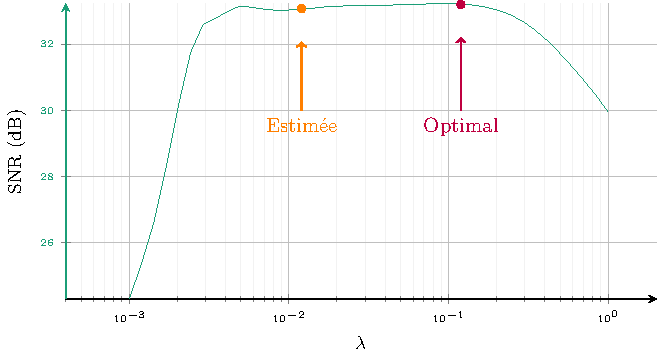
\includegraphics{img/chapitre4/figure14/cls-parameter.pdf}
    \caption{Procéssus d'estimation du paramètre de CLS. $\mathsf{R}_2^*$ est reconstruit à l'aide de CLS pour un ensemble de valeurs de paramètre et le SNR est calculé pour chaque valeur de $\lambda$. Le paramètre ajusté par le processus dichotomique est indiqué d'un point orange tandis que le paramètre optimal, \ie{}, celui conduisant à la meilleure reconstruction, est affiché en rouge. Ce résultat montre que la stratégie proposée afin d'ajuster automatiquement le paramètre de régularisation donne des performances de reconstruction proches des valeurs optimales.
        \protect\label{fig-lambda_estim}}
\end{figure}


\section{Reconstruction dans le cas d'un bruit mixte poisson-gaussien}\label{sec-bruit-mixte}

Dans les expériences conduites à la section~\ref{sec-hr-results}, les images semi-réelles sont corrompues par un bruit blanc additif gaussien. Toutefois, cette hypothèse peut être remise en question puisque les données spectroscopiques en microscopie sont sencés être corrompus par un bruit mixte poisson-gaussien, comme détaillé à la section~\ref{sec-nature-bruit}. Puisqu'il est difficile de déduire la proportion des deux composantes à l'origine du bruit composant le mélange, seule la composante gaussienne a été conservée dans les expériences.

Pour souligner la robustesse de CLS dans le cas d'un bruit mixte poisson-gaussien, l'image non-bruitée $\bar{\mathsf{R}}_2$ a été dégradée en suivant les deux procédures suivantes :
\begin{itemize}
    \item $\mathcal{P}_{\mathrm{G}}$ : un bruit additif gaussien de variance $\sigma^2$ a été ajouté à $\bar{\mathsf{R}}_2$ afin de construire l'image corrompue $\mathsf{R}_2^{(\mathrm{G})}$,
    \item $\mathcal{P}_{\mathrm{PG}}$ : un bruit poissonnien de variance $\sigma^2/2$ a été appliqué à $\bar{\mathsf{R}}_2$, suivi d'un bruit additif gaussien de variance $\sigma^2/2$ afin d'obtenir l'image corrompue notée $\mathsf{R}_2^{(\mathrm{PG})}$.
\end{itemize}
Notons que les deux images corrompues $\mathsf{R}_2^{(\mathrm{G})}$ et $\mathsf{R}_2^{(\mathrm{PG})}$ présentent le même niveau de bruit total $\sigma^2$. Elles sont sous-échantillonnées avec un taux d'échantillonnage de 20\%, puis reconstruites en utilisant NN, 3S et CLS. Les performances de reconstruction en termes de SNR sont données à la \tabname~\ref{table:SNR-poisson-gaussian} pour deux niveaux de bruit $\sigma^2$. Ces résultats montrent que les performances de la méthode ne sont pas significativement dégradées lorsque l'on considère un modèle de bruit plus réaliste.

\begin{table}[t]
    \centering
    \begin{tabular}{ccc|cc}
        \toprule
        & \multicolumn{2}{c|}{$\sigma^2$} & \multicolumn{2}{c}{$10^4\times\sigma^2$}\\
        %
        & $\mathcal{P}_{\mathrm{G}}$ & $\mathcal{P}_{\mathrm{PG}}$ & $\mathcal{P}_{\mathrm{G}}$ & $\mathcal{P}_{\mathrm{PG}}$\\
        \midrule
        NN     & 28,71    & 28,71              & 25,17    & 24,85 \\
        3S     & 30,17    & 30,18              & 28,02    & 28,05 \\
        CLS    & 33,15    & 33,15              & 29,05    & 28,67 \\
        \bottomrule
    \end{tabular}
    \caption{Performances de reconstruction en termes de SNR (dB) pour les images $\mathsf{R}_2^{(\mathrm{G})}$ et $\mathsf{R}_2^{(\mathrm{PG})}$. Les résultats sont similaires pour les deux procédures de corruption $\mathcal{P}_{\mathrm{G}}$ et $\mathcal{P}_{\mathrm{PG}}$, ce qui montre que CLS n'est pas particulièrement impacté par le bruit poissonnien.
        \protect\label{table:SNR-poisson-gaussian}}
\end{table}


\section{Création des spectre-images synthétiques et semi-réels}\label{sec-spim-creation-hr}

\paragraph{Synthèse du spectre-image synthétique $\mathsf{S}$.} Pour générer le spectre-image synthétique $\mathsf{S}$, la stratégie utilisée à la section~\ref{sec-synth-data-lr} sera utilisée. Cela consiste à réaliser un mélange linéaire de $N_c=4$ composantes suivant des cartes d'abondances réalistes. Les composantes spectrales ont été obtenues en lissant $N_c$ signatures identifiées par \gls{aci} à partir du spectre-image réel $\mathsf{R}_2$. Elles sont rassemblées dans la matrice $\gls{M}$ de taille $\gls{M}\times N_c$ est sont représentées à la figure~\ref{fig-spectra-synth}. Les cartes d'abondances sont générées synthétiquement en superposant une structure périodique avec un fond évoluant doucement de manière similaire au spectre-image réel $\mathsf{R}_2$. Ces cartes rassemblées dans la matrice \gls{A} de taille $N_c\times\gls{P}$ sont représentées à la figure~\ref{fig-maps-synth}. Enfin, l'image synthétique $\mathsf{S}$ est obtenue en calculant $\gls{Mu}\gls{A}$.

\begin{figure}[b]
    \centering
    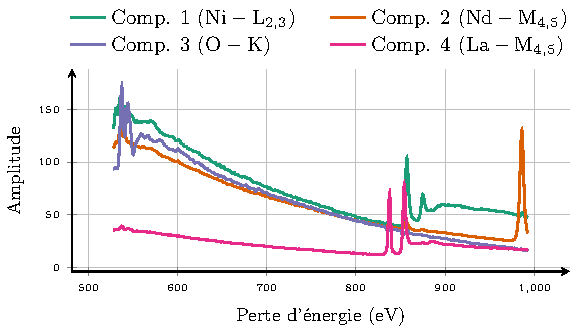
\includegraphics{img/chapitre4/figure16/synth_spectra.pdf}
    \caption{Composantes spectrales utilisées pour générer l'image synthétique $\mathsf{S}$.
        \protect\label{fig-spectra-synth}}
\end{figure}

\begin{figure}[t]
    \centering
    \setlength\tmplength{5cm}
    \subfigure[Comp. 1]{
\includegraphics[width=\tmplength]{img/chapitre4/figure16/data/map_0.png}}
    \subfigure[Comp. 2]{
\includegraphics[width=\tmplength]{img/chapitre4/figure16/data/map_1.png}}
    \subfigure[Comp. 3]{
\includegraphics[width=\tmplength]{img/chapitre4/figure16/data/map_2.png}}
    \subfigure[Comp. 4]{
\includegraphics[width=\tmplength]{img/chapitre4/figure16/data/map_3.png}}
    \caption{Cartes d'abondance associées aux composantes spectrales représentées à la figure~\protect\ref{fig-spectra-synth} utilisées pour générer le spectre-image synthétique $\mathsf{S}$.
        \protect\label{fig-maps-synth}}
\end{figure}


\paragraph{Création des spectre-images semi-réels $\mathsf{R}_1^*$ et $\mathsf{R}_2^*$.} Les spectre-images non-bruités $\bar{\mathsf{R}}_1$ et $\bar{\mathsf{R}}_2$ utilisés à la section~\ref{sec-results-hr-synth} sont générés en ne conservant que les $R$ premières composantes principales identifiées par ACP appliqué à $\mathsf{R}_1$ et $\mathsf{R}_2$ respectivement. Dans ces travaux, le seuil $R$ est choisi tel que les $M-R$ composantes restantes ne contiennent pas d'information spatiale. Pour quantifier la présence ou l'absence d'information spatiale dans une composante principale, la blancheur est vérifiée en se basant sur les métriques proposées dans\cite[chap. 3]{riot2018residual} selon
\begin{equation}
    ||r||_2^* = \sqrt{\sum_{\tau\neq 0} r(\tau)^2}
\end{equation}
où $r(\tau)$ est la fonction d'autocorrélation 2D. Plus la valeur est élevée, plus l'image contient d'information spatiale. Pour servir d'illustration, le critère est représenté à la figure~\ref{fig-whiteness-metric} en fonction de l'indice associé à la composante spectrale pour les deux spectre-images $\mathsf{R}_1$ et $\mathsf{R}_2$. Le seuil de l'ACP $R$ est choisi comme l'indice maximum suffisant à atteindre un comportement stationnaire de la courbe. Ces valeurs sont reportées à la \tabname~\ref{table-hr-samples}. Les spectre-images semi-réels $\mathsf{R}_1^*$ et $\mathsf{R}_2^*$ sont finallement obtenus en altérant les spectres-images non-bruités $\bar{\mathsf{R}}_1$ et $\bar{\mathsf{R}}_2$ avec des bruits blancs additifs gaussiens dont les variances ont été ajustés pour atteindre des valeurs de SNR en accord avec ceux des spectre-images de référence correspondants $\mathsf{R}_1$ et $\mathsf{R}_2$ respectivement.

\begin{figure}[]
    \centering
    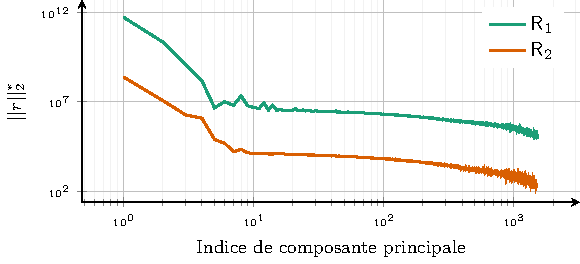
\includegraphics{img/chapitre4/figure17/remaining_structure.pdf}
    \caption{Critère de blancheur  $||r||_2^*$ en fonction de l'indice de composante principale pour les images réelles $\mathsf{R}_1$ et $\mathsf{R}_2$. Les premières composantes principales de puissance supérieure présentent plus de contenu spatial que les dernières composantes. Le seuil de l'ACP choisi est l'indice maximal suffisant pour atteindre un comportement stationnaire de la courbe.
        \protect\label{fig-whiteness-metric}}
\end{figure}



\section{Correction de CLS par refitting}

Dans la section~\ref{s2n-formulation}, la méthode proposée S2N favorise les images de rang faible en contraignant la norme nucléaire du spectre-image. De même, la méthode CLS proposée à la section~\ref{sec-formulation-cls} promeut les représentations parcimonieuses dans la base DCT à l'aide de la norme $\ell_{1}$. Ces deux normes proposées comme relaxations convexes du rang et de la pseudo-norme $\ell_0$ respectivement ne sont cependant pas optimales puisqu'elles introduisent un biais systématique dans les images reconstruites.

Pour corriger ce biais, des travaux ont proposé de raffiner l'estimée \gls{Xh} obtenue en vue d'obtenir une estimée $\tilde{\mathbf{X}}$ moins biaisée sans altérer les propriétés d'intérêt de \gls{Xh}, cette approche est appelée \emph{refitting}. %
%
Par exemple, dans~\cite{deledalle2017clear}, les auteurs proposent de conserver l'information contenue dans le Jacobien de \gls{Xh} en vue de raffiner de nombreux problèmes traités en traitement du signal.


Si l'on s'intéresse plus préscisément à CLS pour lequel \gls{Xh} présente une parcimonie groupée dans la base DCT, une première méthode simple consiste à ré-estimer la solution sur le support de la représentation de \gls{Xh} seulement.
Plus précisément, si l'on note $\hat{\Gamma}$ (resp. $\tilde{\Gamma}$) le support de la représentation parcimonieuse de \gls{Xh} (resp. $\tilde{\mathbf{X}}$), l'image raffinée devra respecter $\tilde{\Gamma} \subseteq \hat{\Gamma}$. En ce qui concerne CLS, le support s'écrit%
%
\footnote{Afin d'alléger les notations, nous considérons que les données n'ont pas été traité ACP en pré-traitement. Toutefois, cette décomposition est réalisée dans les expériences décrites dans cette section.}
%
\begin{equation}
    \hat{\Gamma} = \mathrm{supp}(\gls{Xh}\Psi)  = \{p\ :\ (\gls{Xh}\Psi)_p \neq \mathbf{0}_M \}.
\end{equation}
Plus présisément, nous pouvons implémenter une correction par MC contraints comme dans~\cite{belloni2013least}, ce qui donnerait pour CLS
\begin{equation}
    \tilde{\mathbf{X}} = \argmin_{\gls{X} : \mathrm{supp}(\gls{X}\Psi)\subseteq\hat{\Gamma}} 
    %
    \frac{1}{2}\frobnorm{\gls{Y}_{\gls{I}} - \gls{X}_{\gls{I}}}
\end{equation}
ou encore, après réécriture,
\begin{equation}\label{eq-refining-simple}
    \tilde{\mathbf{X}} = \argmin_{\gls{X}} 
    %
    \frac{1}{2}\frobnorm{\gls{Y}_{\gls{I}} - \gls{X}_{\gls{I}}} + 
    %
    \sum_{p\in\hat{\Gamma}^c} \iota_{\{\mathbf{0}_M\}}((\gls{X}\Psi)_p)
\end{equation}
où $\hat{\Gamma}^c$ correspond à l'ensemble des indices n'appartenant pas au support de \gls{Xh}. Cette méthode appelée \emph{post-MC} nécessite tout de même que le nombre de positions visitées $N$ soit supérieur à $|\hat{\Gamma}|$ pour s'assurer que le problème soit bien posé.

Cette méthode, bien que simple, a toutefois l'inconvénient d'être fortement instable et des travaux ont proposé de conserver, en plus du support $\hat{\Gamma}$ de \gls{Xh}, davantage de caractéristiques inhérentes à \gls{Xh}. Dans~\cite{deledalle2019block}, les auteurs ont ainsi suggéré que les composantes non-nulles des représentations de \gls{Xh} et $\tilde{\mathbf{X}}$ partagent la même direction, voire la même orientation. Plus précisément, en définissant le cosinus de deux vecteurs $v$ et $v'$ dans $\mathbb{R}^M$ par
\begin{equation}
    \cos(v, v') = \left< \frac{v}{||v||_2} , \frac{v'}{||v'||_2} \right> = \frac{1}{||v||_2\cdot||v'||_2}\sum_k v_kv_k',
\end{equation}
l'image corrigée est dite conserver la direction (D) si 
\begin{equation}
    \cos( (\tilde{\gls{X}}\Psi)_p , (\gls{Xh}\Psi)_p ) = \pm 1 \qquad \forall p\in\hat{\Gamma}
\end{equation}
et est dite conserver l'orientation (O) si le cosinus vaut 1. Ces deux contraintes sont mises en \oe{}uvre à l'aide de pénalisations faibles (notées SD et SO), quadratiques (QD, QO) et fortes (HD, HO). Ces régularisations notées $\phi$ sont finalement incluses dans le problème d'optimisation~\ref{eq-refining-simple} pour donner
\begin{equation}
\tilde{\mathbf{X}} = \argmin_{\gls{X}} 
%
\frac{1}{2}\frobnorm{\gls{Y}_{\gls{I}} - \gls{X}_{\gls{I}}} + 
%
\sum_{p\in\hat{\Gamma}^c} \iota_{\{\mathbf{0}_M\}}((\gls{X}\Psi)_p) +
%
\sum_{p\in\hat{\Gamma}} \phi( (\gls{X}\Psi)_p , (\gls{Xh}\Psi)_p ).
\end{equation}
Cette méthode appelée \emph{block-based refitting} (BBR) sera notée BBR-SD, BBR-So, etc. suivant la régularisation utilisée.

Les performances de ces méthodes de refitting sont évaluées lors de la reconstruction de $\mathsf{R}_2^*$ et de $\mathsf{S}^*$ pour un taux d'échantillonnage de 20\%. Les résultats sont donnés à la \tabname~\ref{table-refitting} pour touts les méthodes étudiée au chapitre~\ref{ch-chapter_4} et pour les techniques de refitting.
%
On observe d'abord que les approches par refitting se classent, comme CLS, entre les méthodes d'interpolation (et 3S) et les méthodes par \gls{ad} en termes de performances. 
%
Ensuite, comme attendu, les approches par reffiting affichent un SNR supérieur à CLS pour l'image $\mathsf{S}^*$ et les performances de BBR sont même meilleures que celles de post-MC.
%
Cela encourage l'utilisation des approches par reffiting et montre l'intérêt à conserver l'information issue de \gls{Xh} pour évaluer $\tilde{\mathbf{X}}$. 
%
Toutefois, ces observations ne tiennent plus avec l'image semi-réelle $\mathsf{R}_2^*$ puisque les méthodes par refitting affichent des performances moindres par rapport à CLS, tout particulièrement post-MC qui perd \np[dB]{0.7}. 
%
Cela tend à montrer que la norme $\ell_{2, 1}$ est suffisante pour notre application et que l'algorithme CLS est suffisamment performant en reconstruction d'images STEM-EELS sous-échantillonnées.


\begin{table}
    \centering
    \bgroup
    \renewcommand{\arraystretch}{1,2}
    %
    \begin{tabular}{*{3}{M{2cm}}}%
        \toprule
        \multirow{2}{*}{Méthode}& \multicolumn{2}{c}{SNR}\\
        %
        &$\mathsf{R}_2^*$&$\mathsf{S}^*$\\
        %
        \midrule
        %
        NN          & 28,71 & 21,32 \\
        3S          & 30,17 & 22,12 \\
        \midrule
        CLS         & 33,15 & 42,14 \\
        post-MC     & 32,45 & 42,22 \\
        BBR-HO      & 33,07 & 42,36 \\
        BBR-HD      & 33,07 & 42,36 \\
        BBR-QO      & 32,75 & 42,40 \\
        BBR-QD      & 32,80 & 42,40 \\
        BBR-SO      & 33,07 & 42,36 \\
        BBR-SD      & 32,78 & 42,38 \\
        \midrule
        ITKrMM      & 33,67 & 44,16 \\
        wKSVD       & 34,52 & 45,59 \\
        BPFA        & 35,01 & 52,70 \\
        %
        \bottomrule
    \end{tabular}
\egroup
    \caption{Performances en reconstruction des méthodes par refitting en termes de SNR pour l'image semi-réelle $\mathsf{R}_2^*$ et pour l'image synthétique $\mathsf{S}^*$. Les performances des méthodes utilisées au chapitre~\ref{ch-chapter_4} sont également affichées pour comparaison.
        \protect\label{table-refitting}}
\end{table}







